\documentclass{article}
\usepackage[utf8]{inputenc}
\usepackage{graphicx}
\usepackage{float}
\usepackage[left=20mm, right=20mm, top=2mm, bottom=20mm]{geometry}



\title{Is Florida getting warmer?}
\author{Agnes Szwarczynska\, aas122@ic.ac.uk} 
\date{\today}



\begin{document}
    \maketitle

    \section{Introduction}

   The aim of this practical was to investigate whether there is any correlation between the temperatures and years in the 20th century in Key West in Florida, USA.

    \section{Materials \& Methods}
    
    The true (pearson) correlation coefficient has been calculated using EcolArchives-E089-51-D1.csv data file containing set of annual temperatures in Key West in Florida, USA from the 20th century. The distribution of generated correlation coefficients has been produced by randomly re-assigning temperatures to years 10000 times. The true correlation coefficient was then plotted against the distribution - a standard p-value could not be used in this case since measurements of climatic variables across successive years are not independent from each other.
    

    \section{Results}
    
\begin{figure}[H]
\centering
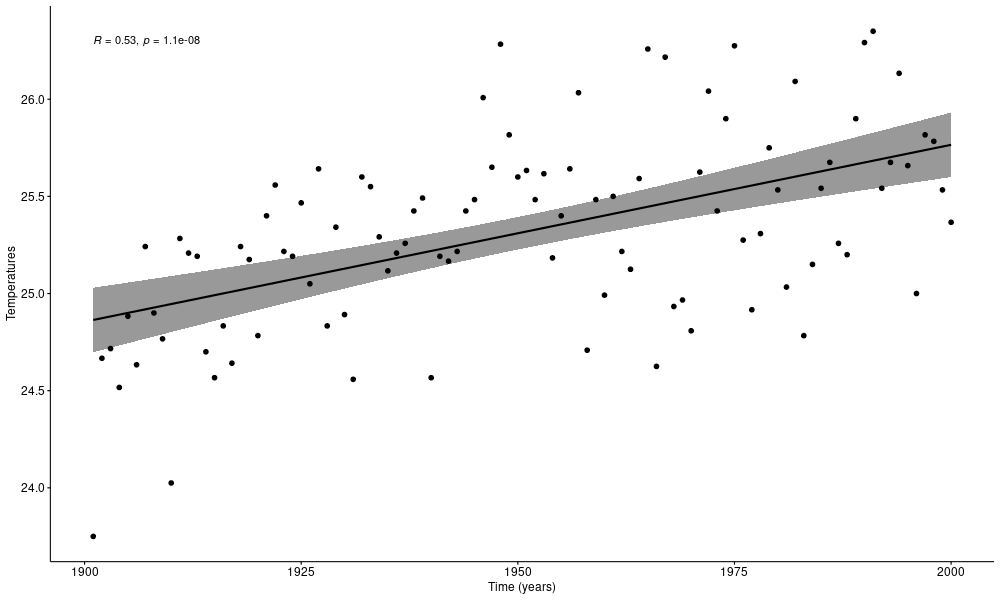
\includegraphics[scale=0.2]{../data/plot1.png}
\caption{Temperatures in the 20th century in in Key West in Florida, USA }
\end{figure}

\begin{figure}[H]
\centering
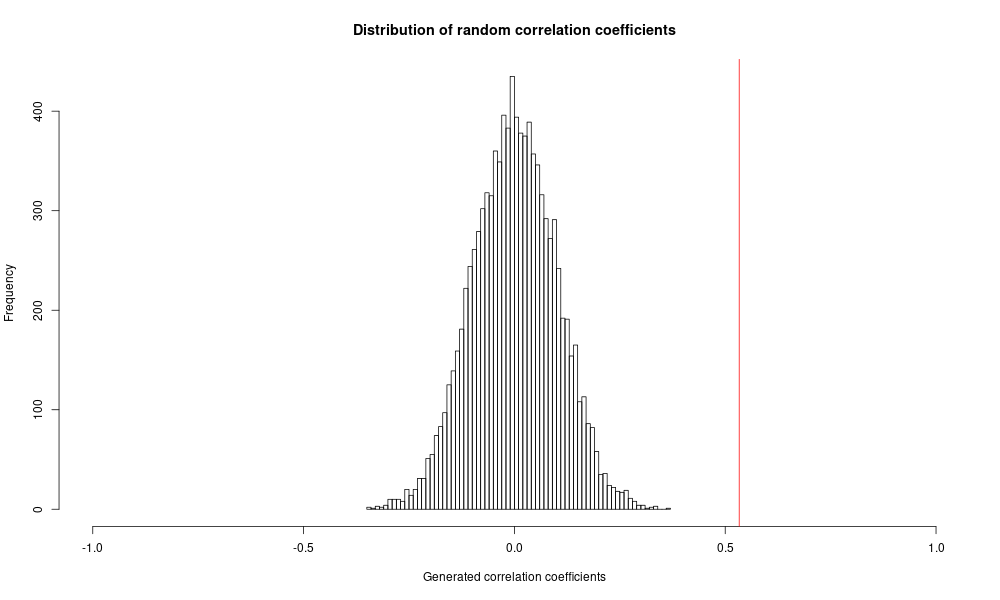
\includegraphics[scale=0.2]{../data/histogram1.png}
\caption{Distribution of randomly generated correlation coefficients. Red line depicts the true correlation coefficient from the original dataset.}
\end{figure}
    
    \section{Discussion}
    
    After calculating what fraction of the random correlation coefficients were bigger than the original one (asymptotic p-value was smaller than 0.001) and visually assessing the histogram, we can conclude that temperatures in the past century have been continuously increasing in Florida. 

\end{document}